\documentclass{article}
\usepackage[utf8]{inputenc}
\usepackage[shortlabels]{enumitem}

\title{Problem Set 2 Solution Template}
\author{Xiaoli Sun (xs2338)}
\date{Sep.26 2020}

\usepackage{natbib}
\usepackage{graphicx}
\usepackage{float}

\begin{document}

\maketitle

\section*{Problem 1: Installment Loan Terms and Trade-offs}


\begin{enumerate}[(a)]
   \item See table below. \\
   Python code:
   \begin{verbatim}
#the value of m and r can change
m= 72
r = 2/100
P = 25000
M = ((1/m)+0.5*(r/12)+(1/8)*(m-2)*(r/12)*(r/12))*P
Interest_paid = M*m-P
DTI = M*12/50000
\end{verbatim}

   \begin{enumerate}[(i)]
       \item  Monthly payments $ = \mathit{M}=P \times{(\sum_{i=1}^{m}\frac{1}{{(1+r_{loan}/12)}^i})}^{-1}$ \\
       $\approx \approx  P \times [\frac{1}{m}+\frac{1}{2}(r_{loan}/12)+\frac{1}{8}(m-2){(r_{loan}/12)}^2]$ 
       \item Total interest paid over the life of the loan $ = M \times m - P$
       \item DTI (debt-to-income) change for your cousin assuming an income of \$50, 000 annually=
       $DTI = \frac{monthlydebt}{\frac{50,000}{12}}$
      
   \end{enumerate}

\begin{table}[H]
    \centering
    
    \begin{tabular}{c|c|c|c|c|c}
    
        \hline
                  &             & (i) & (ii)  & (iii)  \\
        Loan Term & Lowest Rate & Monthly Payment & Total Interest Paid & DTI change  \\ \hline
        36 months &3.00\%  &  726.3585069444445 &  1148.90625 &  0.17432604166666668 \\ \hline
        60 months & 4.50\% & 466.0904947916666&  2965.4296874999927&   0.11186171874999998\\ \hline
        72 months & 2.00\% & 368.6631944444444 & 1543.7499999999964  &0.08847916666666666   \\  \hline
    \end{tabular}
\end{table}

   \item I recommend loan term 72 months with the lowest monthly payment and lowest DTI. It is more flexible. The total interest paid is acceptable. Only 400\$ higher than 36-month term, but has a much more low DTI and monthly payment. 
   
   \item 
   
      \begin{enumerate}[(i)]
       \item ""
       
\begin{table}[H]
    \centering
    \begin{tabular}{c|c|c|c}
        \hline
        Loan Term & New/Lower Loan Rate & Monthly Payment Savings & Total Interest Savings \\ \hline
        36 months &  2.90\%& 1.0851996527778738 & 39.067187500004366  \\ \hline
        60 months & 4.40\% &1.153689236111063 &  69.22135416666379 \\ \hline
        72 months & 1.90\%  & 1.1009114583333144 &  79.26562499999864 \\  \hline
    \end{tabular}
\end{table}
       
       \item Python code:
       \begin{verbatim}
#M = Original Monthly Payment+25
m = 72
r = 2/100
M = 368.6631944444444+25
P = M*m/((1+r/12)**(m/2))
\end{verbatim}

\begin{table}[H]
    \centering
    \begin{tabular}{c|c|c|c|c}
        \hline
        Loan Term & Loan Rate & Original Monthly Payment & New Monthly Payment & New Principal  \\ \hline
        36 months &  3.00\% &726.3585069444445 & 751.3585069444445  &  25860.138433500404\\ \hline
        72 months & 2.00\%  & 368.6631944444444 & 393.6631944444444 & 26694.471707895496 \\  \hline
    \end{tabular}
\end{table}
       
       \item Python code:
       \begin{verbatim}
M=368.6631944444444
m=84
r=2/100
P = M*m/((1+r/12)**(m/2))
\end{verbatim}
$P = 28875.78236902694$

       
   \end{enumerate}

   
 \end{enumerate}

\newpage
\section*{Problem 2: Lending Club Loan Examples}

\begin{enumerate}[(a)]
   \item Python code:
\begin{verbatim}
import pandas as pd 
#import data
df = pd.read_csv("/Users/liloli/Desktop/GR5293/hw2/LendingClub_2016Q1.csv") 
# pick the first four loans with different grades
df_a = df[df['grade']=='A']
row_a = df_a.head(1)
df_b = df[df['grade']=='B']
row_b = df_b.head(1)
df_c = df[df['grade']=='C']
row_c = df_c.head(1)
df_d = df[df['grade']=='D']
row_d = df_d.head(1)
table = pd.concat([row_a, row_b, row_c, row_d])
#calculate total interest due
table['total_interest_due'] = table['installment']*36-table['loan_amnt']
#select columns needed
table = table[['loan_amnt', 'int_rate', 'installment','grade',  'sub_grade', 
'total_interest_due']]
display(table.transpose())
\end{verbatim}

   
   \begin{enumerate}[(i)]
       \item Table from python output.
          
    \begin{figure}[h!]
    \centering
    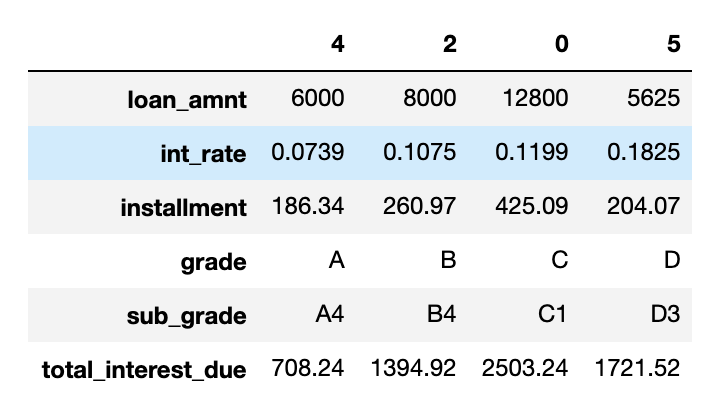
\includegraphics[scale=0.50]{hw2Problem2_a}
    \caption{result}
    \label{fig:original fico_hist}
    \end{figure}
       

 
   

       
   \end{enumerate}
   
   \item Python code:
   \begin{verbatim}
# Begin example
# You might be interested in loans with relatively low installments and low interest rates
# You could look at a distribution of interest rates and then look for loans with certain target rates.
# After filtering out loans outside of the desired range, you can examine 

# Look at a distribution plot of 'int_rate'
import seaborn as sns
sns.distplot(df['int_rate']);
\end{verbatim}
\begin{figure}[h!]
    \centering
    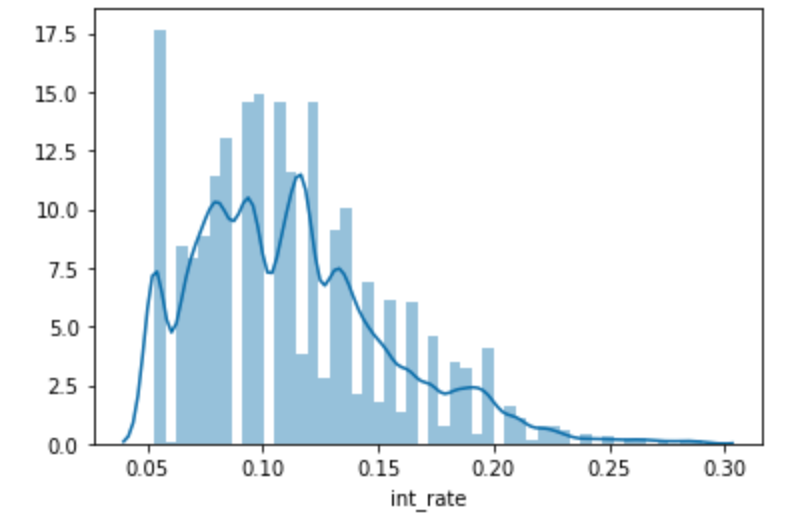
\includegraphics[scale=0.50]{seaborn}
    \caption{A distribution plot of interest rate}
    \label{fig:original fico_hist}
    \end{figure}

Select loans of grade A: Python code
\begin{verbatim}
mydata = df[df['grade']=='A']
mydata.head()
\end{verbatim}

\begin{figure}[h!]
    \centering
    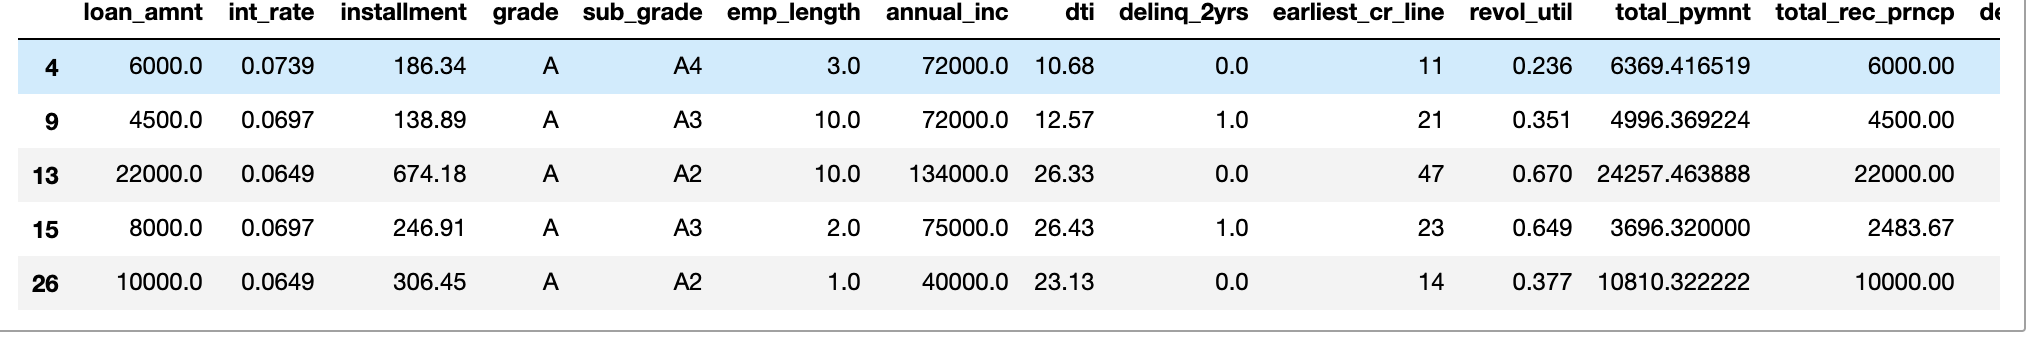
\includegraphics[scale=0.50]{gradeA}
    \caption{grade A loans}
    \label{fig:original fico_hist}
    \end{figure}
    
Describe loans in grade A:\\
Python code:
\begin{verbatim}
mydata.describe()
\end{verbatim}

\begin{figure}[h!]
    \centering
    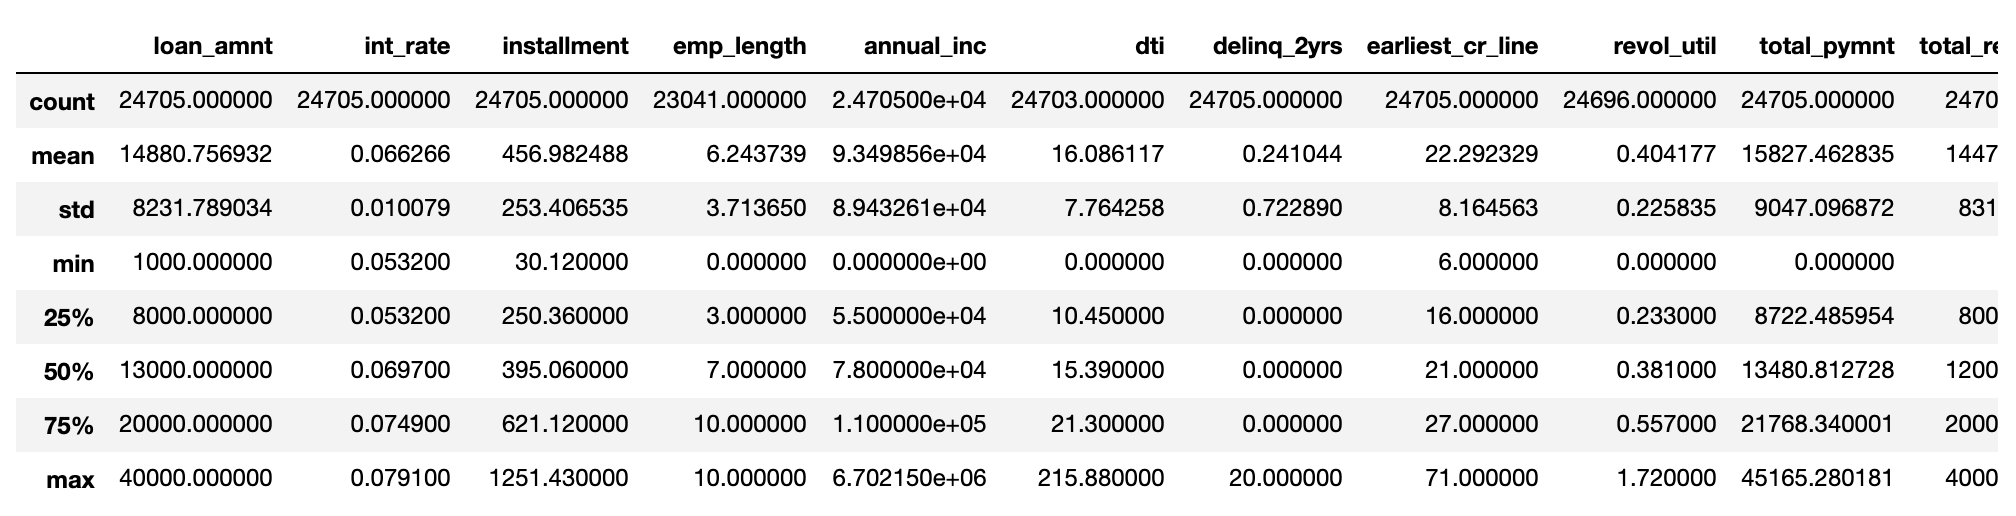
\includegraphics[scale=0.50]{despA}
    \caption{Get initial description of the grade A loans}
    \label{fig:original fico_hist}
    \end{figure}

Distribution of the installment:\\
 Python code:
 \begin{verbatim}
import seaborn as sns
sns.distplot(mydata['installment'])
\end{verbatim}

\begin{figure}[h!]
    \centering
    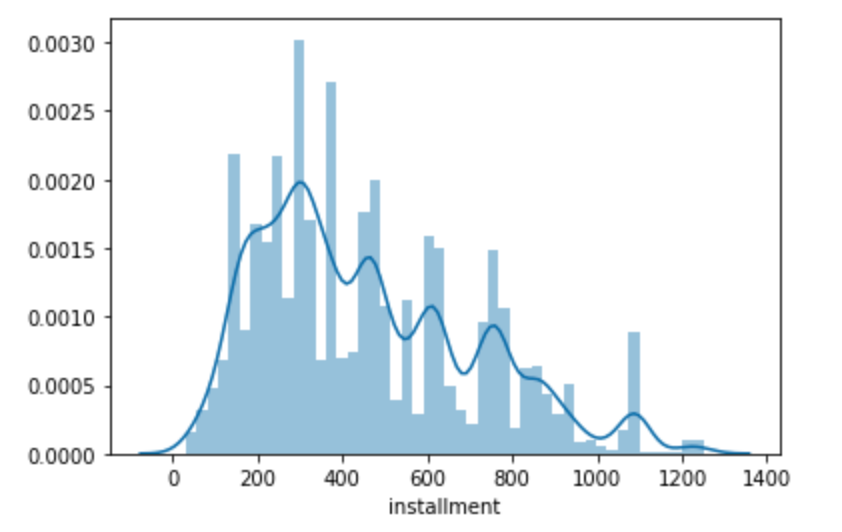
\includegraphics[scale=0.50]{install}
    \caption{Get initial description of the installment}
    \label{fig:original fico_hist}
    \end{figure}
    
 \newpage
    
  \item 
  \textbf{the result table is in the Figure 6}\\
  total-count=96120\\
   Python output table:
  \begin{figure}[h!]
    \centering
    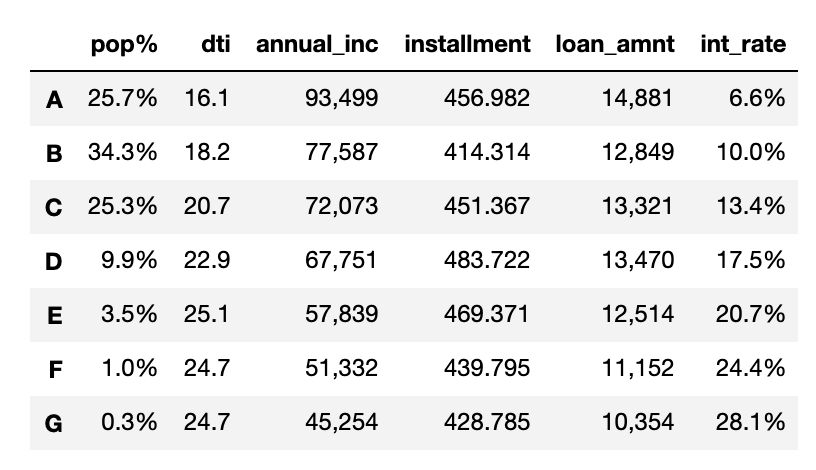
\includegraphics[scale=0.50]{OverviewofLendingClubGrades}
    \caption{Over view of Lending Club Grades}
    \label{fig:original fico_hist}
    \end{figure}


 \end{enumerate}
 
\newpage
\section*{Problem 3: Probability of Default and Loss Given Default from LC Data}
  \begin{figure}[h!]
    \centering
    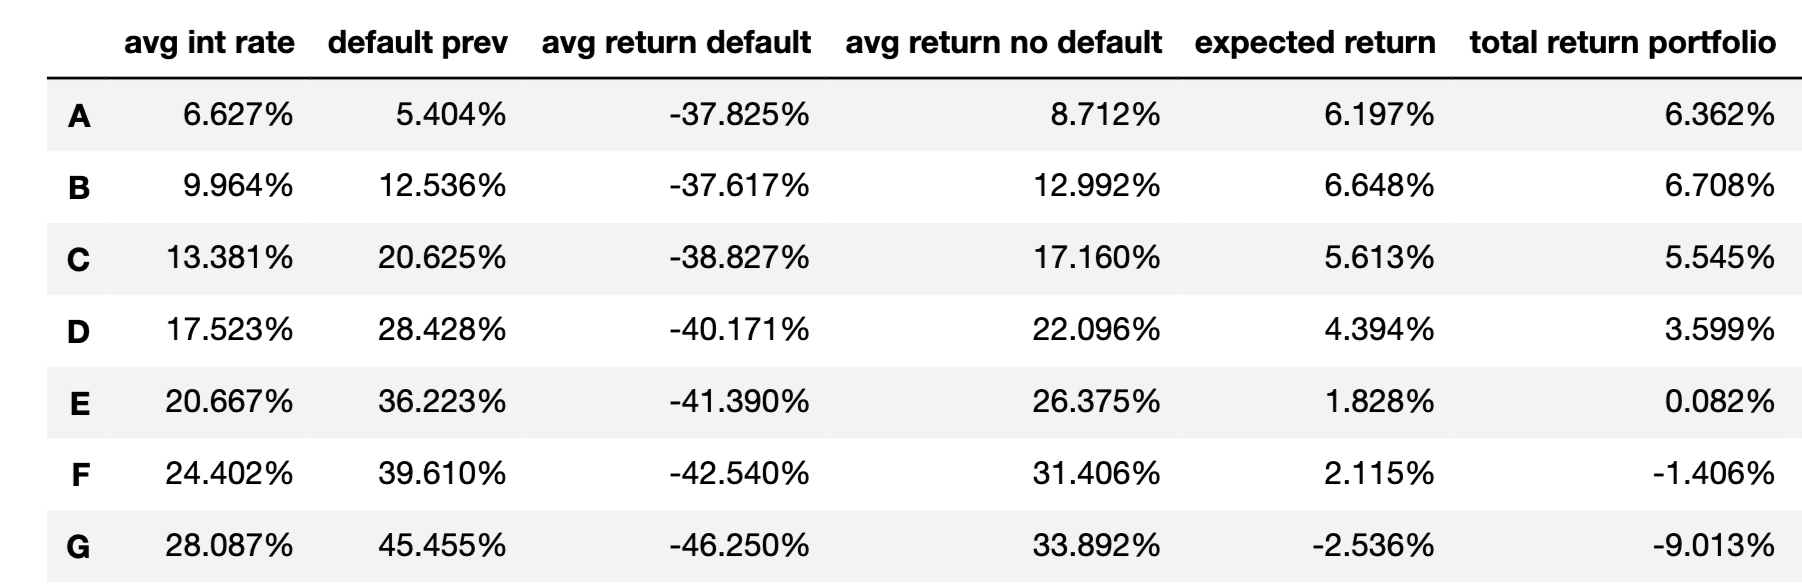
\includegraphics[scale=0.50]{STATs}
    \caption{summarize the results in a table}
    \label{fig:original fico_hist}
    \end{figure}


\begin{enumerate}[(a)]
   \item most favorable portfolio return overall: \textbf{grade B 6.708\%}\\
   the least favorable portfolio return overall: \textbf{grade G -9.013\%}\\
  Which of the two quantities presents a higher variability as the loan grade changes? \\
  Calculate the standard deviation of these two quantities:\\
  Python code:
  \begin{verbatim}
summary_stats[['default prev', 'avg return default']].std()
\end{verbatim}
std(default prev) =         0.147358\\
std(avg return default) =    0.030608\\
\textbf{default prev} presents a higher variability as the loan grade changes.
 
   \item
   
   \begin{enumerate}[(i)]
\item If all loans had the same original loan balance/"loan-amnt", there will be \textbf{NO} difference. \\
\\
$Expected Return  =\\
 \frac{2n_d-n}{n}+\frac{1}{n}\times[\sum_{i \in No Default}\frac{Total LoanPayment_i}{LoanAmount_i}-\sum_{j \in Default}\frac{Total LoanPayment_j}{LoanAmount_j}]$\\
 \\
Expected Return take "Prob of Default" into consideration.
 \\
 \\
 \\
$Portfolio Return = \frac{\sum_{i=1}^{n}TotalPayment_i}{\sum_{i=1}^{n}TotalLoanAmount_i}-1$
 \\
 \\
 Portfolio Return does not take "Prob of Default" into consideration.

\item A-grade and B-grade: larger loans earn more, smaller loans earn less.\\
D-grade and E-grade: larger loans loss mode, smaller loans loss less.\\
\end{enumerate}

   
   \item See table below:
     \begin{figure}[h!]
    \centering
    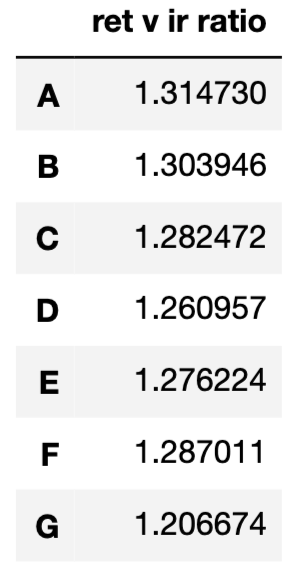
\includegraphics[scale=0.50]{result}
    \caption{Ratio}
    \label{fig:original fico_hist}
    \end{figure}
   
   
 \end{enumerate}
 
\newpage
 
\end{document}

